% You should title the file with a .tex extension (hw1.tex, for example)
\documentclass[a4paper, 11pt]{article}

\usepackage{amsmath}
\usepackage{amssymb}
\usepackage{fancyhdr}
\usepackage{datetime}
\usepackage{graphicx}
\usepackage{scribe}
\usepackage{graphicx}
\usepackage[margin=1in]{geometry}
\usepackage{graphicx}
\newcommand{\question}[2] {\vspace{.25in} \hrule\vspace{0.5em}
\noindent{\bf #1: #2} \vspace{0.5em}
\hrule \vspace{.10in}}
\renewcommand{\part}[1] {\vspace{.10in} {\bf (#1)}}

\newcommand{\myname}{Kriangsak Thuiprakhon, 6080163}
\newcommand{\myemail}{kriangsak.thi@student.mahidol.edu}
\newcommand{\myhwnum}{}
\setlength{\parindent}{0pt}
\setlength{\parskip}{5pt plus 1pt}


\begin{document}

\medskip                        % Skip a "medium" amount of space
                                % (latex determines what medium is)
                                % Also try: \bigskip, \littleskip

\thispagestyle{plain}
\begin{center}                  % Center the following lines
{\Large ICSC302: Final Exam } \\
\myname \\
\myemail \\
\today

\end{center}
\question{1}{What is a double-blind study? Why is it useful? What is the relationship between randomized control trials and double-blind studies?} 

\textbf{\textsc{Answer}}

Blinding or masking refers to the withholding of information regarding treatment allocation from one or more participants in a clinical research study. It is an essential methodological feature of clinical studies that help maximize the validity of the research results.
A \textbf{\textit{double-blind study}}  blinds both the subjects as well as the researchers to the treatment allocation. 

Randomized double blind placebo control (RDBPC) studies are considered the “gold standard” of epidemiologic studies. RDBPC studies remain the most convincing research design in which randomly assigning the intervention can eliminate the influence of unknown or immeasurable confounding variables that may otherwise lead to biased and incorrect estimate of treatment effect. Also, \textit{randomization eliminates confounding by baseline variables and blinding eliminates confounding by co-interventions}, thus eliminating the possibility that the observed effects of intervention are due to differential use of other treatments. The best comparison is placebo control that allows participants, investigators and study staff to be blinded. The advantage of trial over an observational study is the ability to demonstrate causality. 

\question{2}{When can a Binomial Distribution be well approximated by a Poisson Distribution? What is the relationship between Poisson’s $\lambda$ and Binomial’s $N$ and $p$? Do you think the number of traffic deaths per day during Songkran festival is well approximated by a Poisson distribution? Why or why not?}

\textbf{\textsc{Answer}}

\begin{itemize}
\item When the value of $N$ in a binomial distribution is large and the value of $p$ is very small, the binomial distribution can be approximated by a Poisson distribution. If $N > 20$ and $Np < 5$ OR $Nq < 5$ then the Poisson is a good approximation.

\item Poisson's approximation's $\lambda$ parameter to Binomial distribution  is given by:
$$ \lambda = Np$$
\item In 2019's Songkran' holiday 7-day period, Thailand saw 3,724 cases of traffic accidents with a total 418 deaths recorded. The probability of death per day is given by:
$$
P_{death} = 418/3724 = 0.11
$$ 
since   $\lambda = 3724 \cdot 0.11 = 409.64 > 5$, Poisson's approximation should give out a bad approximation.
\end{itemize}
\newpage
\question{3}{During Thailand's holiday seasons such as New Year or Song Kran, traffic deaths seem to increase. If the average number of traffic deaths per day is 30 for non-holidays and is 35 for holidays, do you think there's an actual difference between non-holiday and holiday death rate? Why? Would your conclusion change if the holiday death rate is 40?}

\textbf{\textsc{Answer}}

If the the difference in means is 5 deaths per day, these two sample means may be drawn from the same distribution with some sort of error in sampling, so I do not think that they are two different distributions. However, given that the difference between two means in the second case, which is 10, I think there may be come significant difference, meaning that they may be drawn from different distributions. However, my reasoning is totally based on a personal judgment since I need more data (i.e.,  SDs), of the two means so that I can run a Two-sample t-Test on the two means. 

\question{4}{Find out what homeopathy is. Why is its effectiveness exactly like placebo's?}

\textbf{\textsc{Answer}}

Homeopathy is based on the premise that the substances that cause illnesses can become remedies when highly-diluted in water or an alcohol-based tincture.
Practitioners believe that the molecules retain their memory of the original substance when diluted and rigorously shaken in a process known as ‘poteniation’ or ‘dynamisation’.

A total of 225 existing studies from as far back as 1997 were rated in the NHMRC assessment from one (very strong) to four (very weak) to determine the reliability of their conclusions.

The council found that there is no solid evidence that shows homeopathy being more effective than sugar pills, and other placebos, in making patients feel better and recover.

Chief executive Warwick Anderson says: “There were no health conditions for which there was reliable evidence that homeopathy was effective. For some health conditions, studies reported that homeopathy was not more effective than placebo.

“People who choose homeopathy may put their health at risk if they reject or delay treatments for which there is good evidence for safety and effectiveness,” it added.

Illnesses such as asthma, migraines, stress and colds were tested against homeopathic treatments. Due to lack of evidence, it was found to be not more effective than pretend medicine.


Even though homeopathy has shown some signs of being more effective than placebos for conditions such as ADHD, bruising, HIV, chronic fatigue, ulcers and depression, the experiments were not conducted properly and did not result in very reliable evidence – the report says.

A treatment is considered effective if it causes improvements that cannot be described by the placebo effect and are unlikely to be down to chance. The health improvement has to be significant and continuous for the medicine to be deemed successful – according to the NHMRC.

British and Swiss national health departments have also concluded in the past that homeopathy is not effective enough to be funded by the state. The Australian Homeopathic Association said it was in the process of preparing a formal response to the NHMRC report.

“The Australian Homeopathic Association recommend to the NHMRC that it take a more comprehensive approach to the analysis of homeopathy’s efficacy, and consider a large-scale economic evaluation of the benefits of a more integrated system and one which respects and advocates patient choice in healthcare provision,” the AHA said according to The Guardian.

sources: https://www.independent.co.uk/life-style/health-and-families/health-news/homeopathy-is-not-more-effective-than-placebo-for-almost-every-illness-says-health-council-10099645.html


\question{5}{Estimate the number of cumulative Covid-19 patients for the world and for Thailand on April 30, 2020. Please do some research on how we predict the number of epidemic/pandemic cases before estimating.}

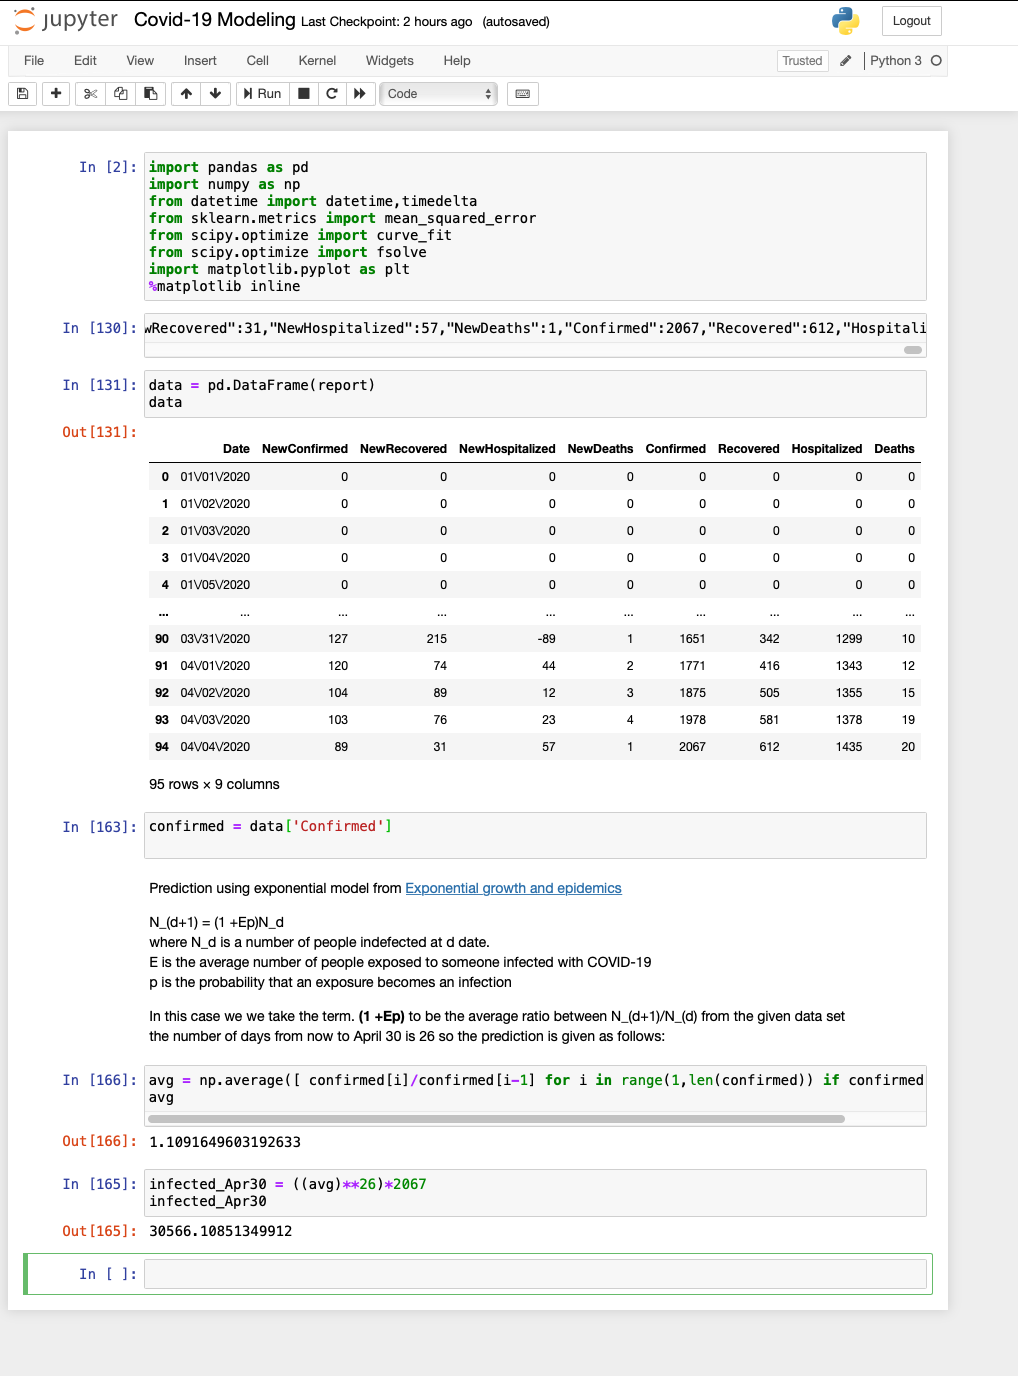
\includegraphics[width=0.8\textwidth]{prediction.png}

\question{6}{Height Estimation}
By trigonometry, the tree height , $\textit{\textbf{h}}$, is given by:
\begin{align*}
h&= ( 1.65 ± 0.05 )  + tan(30 ± 3) \cdot 10.0 ± 1.0 \quad m \\
 &  =  7.42 ± \underbrace{1.71}_{*}  \quad  m \\
 \textmd{*: by Numpy Uncertainty Sampling}
\end{align*}
\end{document}
